\chapter{The choice of the sliding window} % Main chapter title

There is no well-specified procedure for the choice of sliding window $\tau$. Previous studies showed that if $\tau$ is small sub networks become sparse, while for too large sliding windows some important structural changes can not be observed \cite{krings2012effects, arnold2021moving}. We analyse how networks properties and properties of dynamical reputation change with the window size, see SI for more details. Figure A13 in SI shows how considered network properties and dynamical reputation depend on the time window size for active and closed communities on the astronomy. We observe that fluctuations of all measures are more pronounced for time window of 10 days than for 30 and 60 days. However, we find that while the structural properties of networks evolve at different paces over varied time windows the trends remain very similar. The observed qualitative difference between closed and live communities is independent of $\tau$, especially if we compare time window size of 30 and 60 days. The time window size of 30 days ensures enough amount of interaction, even for closed communities, while the number of observation points remains relatively high. For these reasons, we choose a sliding window of 30 days. 

\begin{figure}[h!]
	\centering
	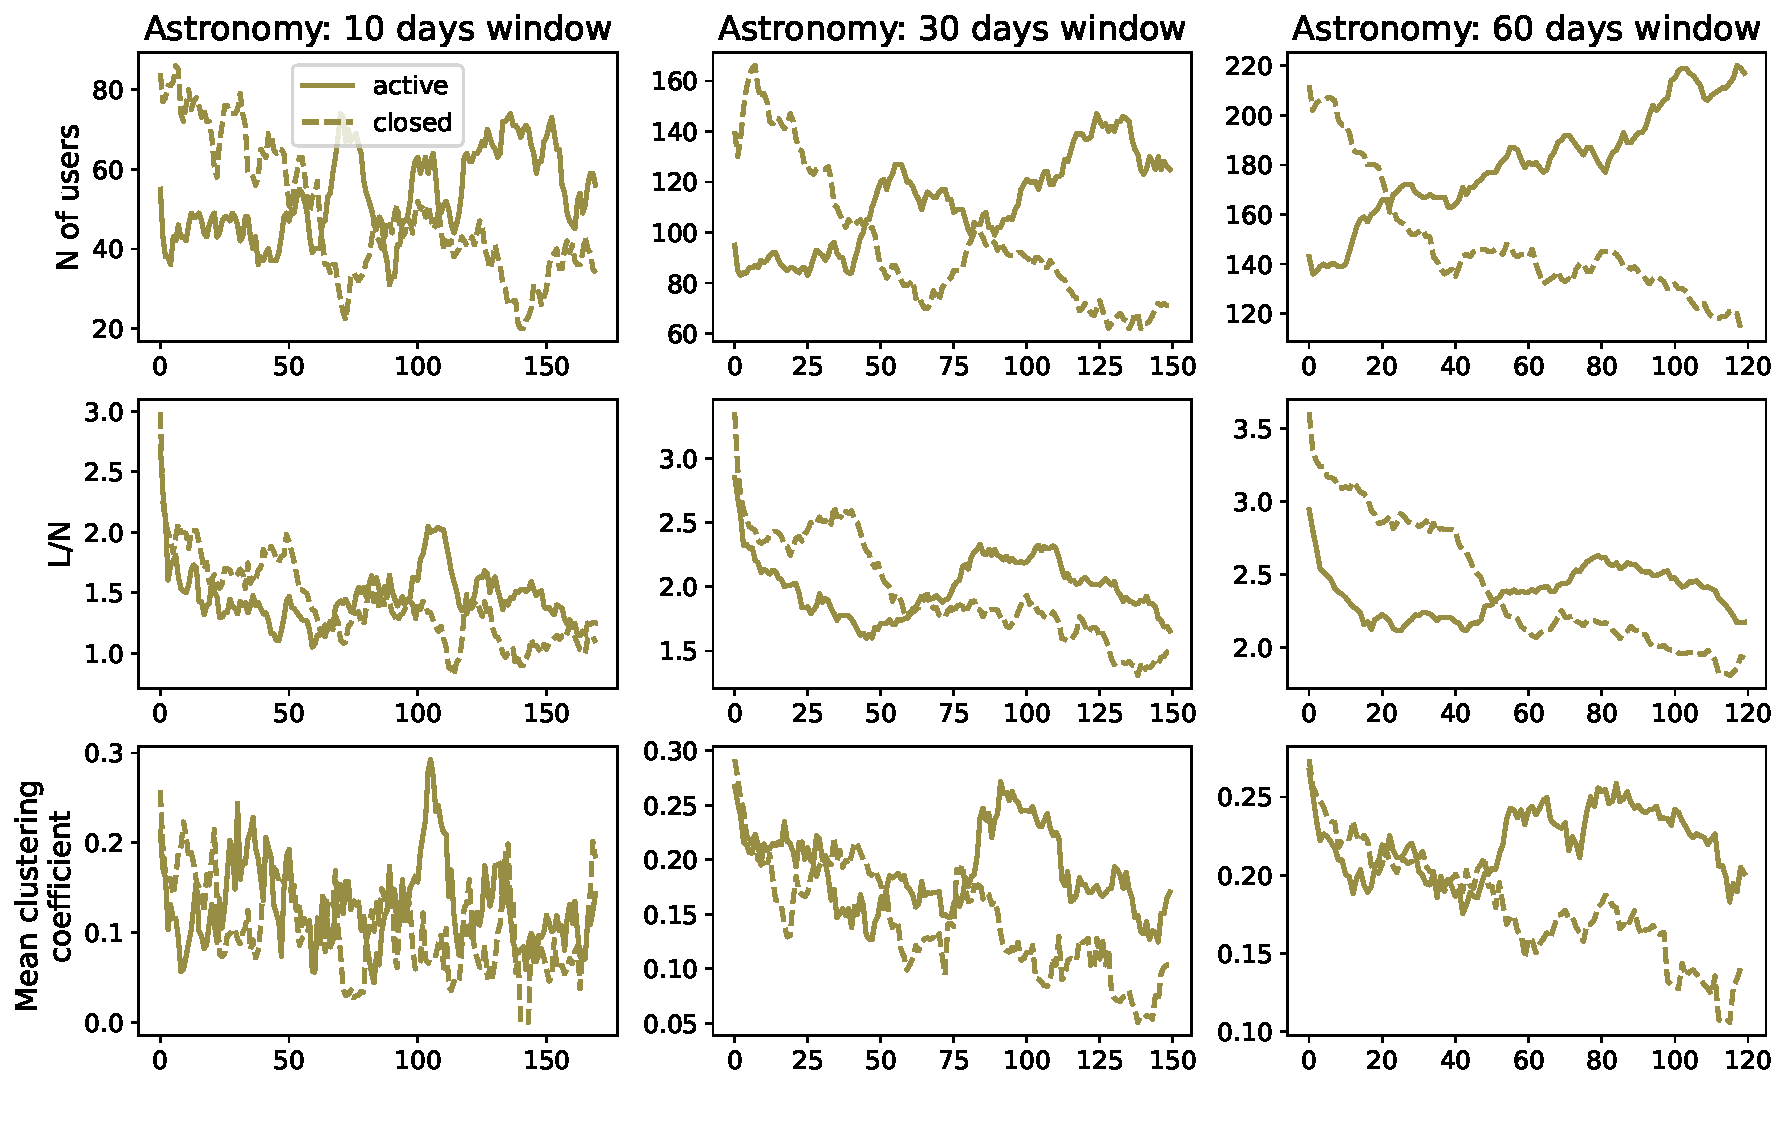
\includegraphics[width=0.9\linewidth]{figures/stackexchange/sliding_window_network.pdf}
	\caption{Results for different sliding windows. Example is for astronomy, blue solid lines- active, orange dashed lines - closed site. }
	\label{fig:windows}
	% Ovo je mozda previse grafika, pa je mozda podeliti na dva dela. 
	% Ovo je primer za astronomiju (ali ako se odlucimo za neku drugu moze se zameniti)
\end{figure}

%ovo neka ide u apendix
In this section, we investigate how the size of sliding windows affect network properties over time. Figure \ref{fig:windows} summarize results for one pair of communities, area51 and beta astronomy, but similar conclusions can be observed for other pairs of sites. We show the network properties for sub-networks of 10, 30, and 60 days sliding windows. For a sliding window of 10 days, results may be too noisy and we may not observe some important trends in the community. The number of users for beta astronomy seems to fluctuate around some mean value. On the larger scale, 30 days window,  it is more clear that the number of users slightly increase over time. Contrary, for too large an aggregation window (60 days), important information about the time series can be lost, such as the local minimum of the number of users around time step 80 that is observed for the 30-day sliding window. Looking into other network characteristics such as L/N and clustering we conclude that differences between closed and  active sites are more transparent with a larger aggregation window, still, on each scale, beta sites show a higher number of nodes, number of links per node and clustering coefficient.

\begin{figure}[h!]
	\centering
	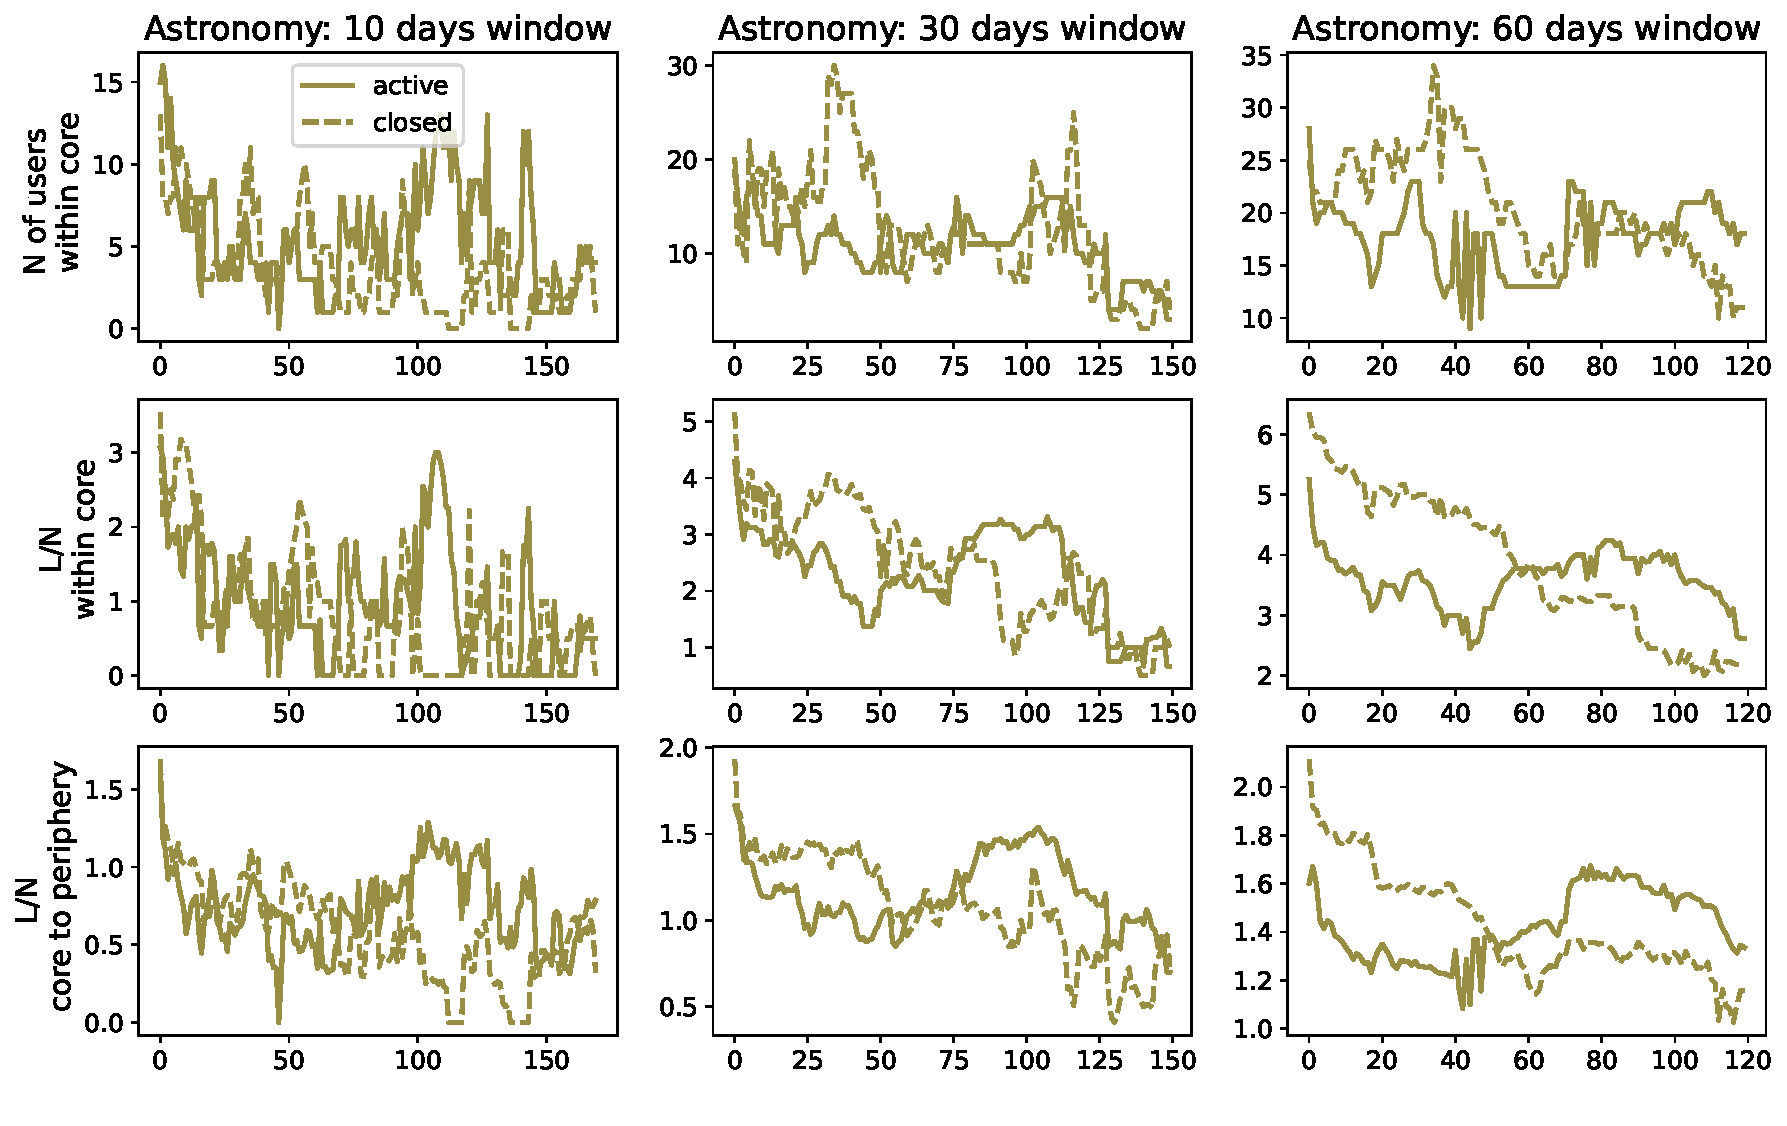
\includegraphics[width=\linewidth]{figures/stackexchange/sliding_window_core_periphery.pdf}
	\caption{Results for different sliding windows. Example is for astronomy, blue solid lines- active, orange dashed lines - closed site. }
	\label{fig:windows}
	% Ovo je mozda previse grafika, pa je mozda podeliti na dva dela. 
	% Ovo je primer za astronomiju (ali ako se odlucimo za neku drugu moze se zameniti)
\end{figure}

As before we study the structure of created sub-networks through the lens of core-periphery structure. On small scales, the window of 10 days, there are often few, or even no nodes in the core and it can affect the calculation of other measures of interest. Such behaviour is more typical for closed communities.  With the size of the sliding window number of nodes in the core increases and results of core-periphery measures %in the number of nodes, L/N in the core, L/N between core-periphery and dynamical reputation between core users and between core and periphery users 
become smoother. Finally, the choice of the sliding window does not change conclusions that core users in the beta communities produce more activity and make the strong core. However, our main results are shown for a sliding window of 30 days, as it makes a good compromise between large and small time scales.  

\begin{figure}[h!]
	\centering
	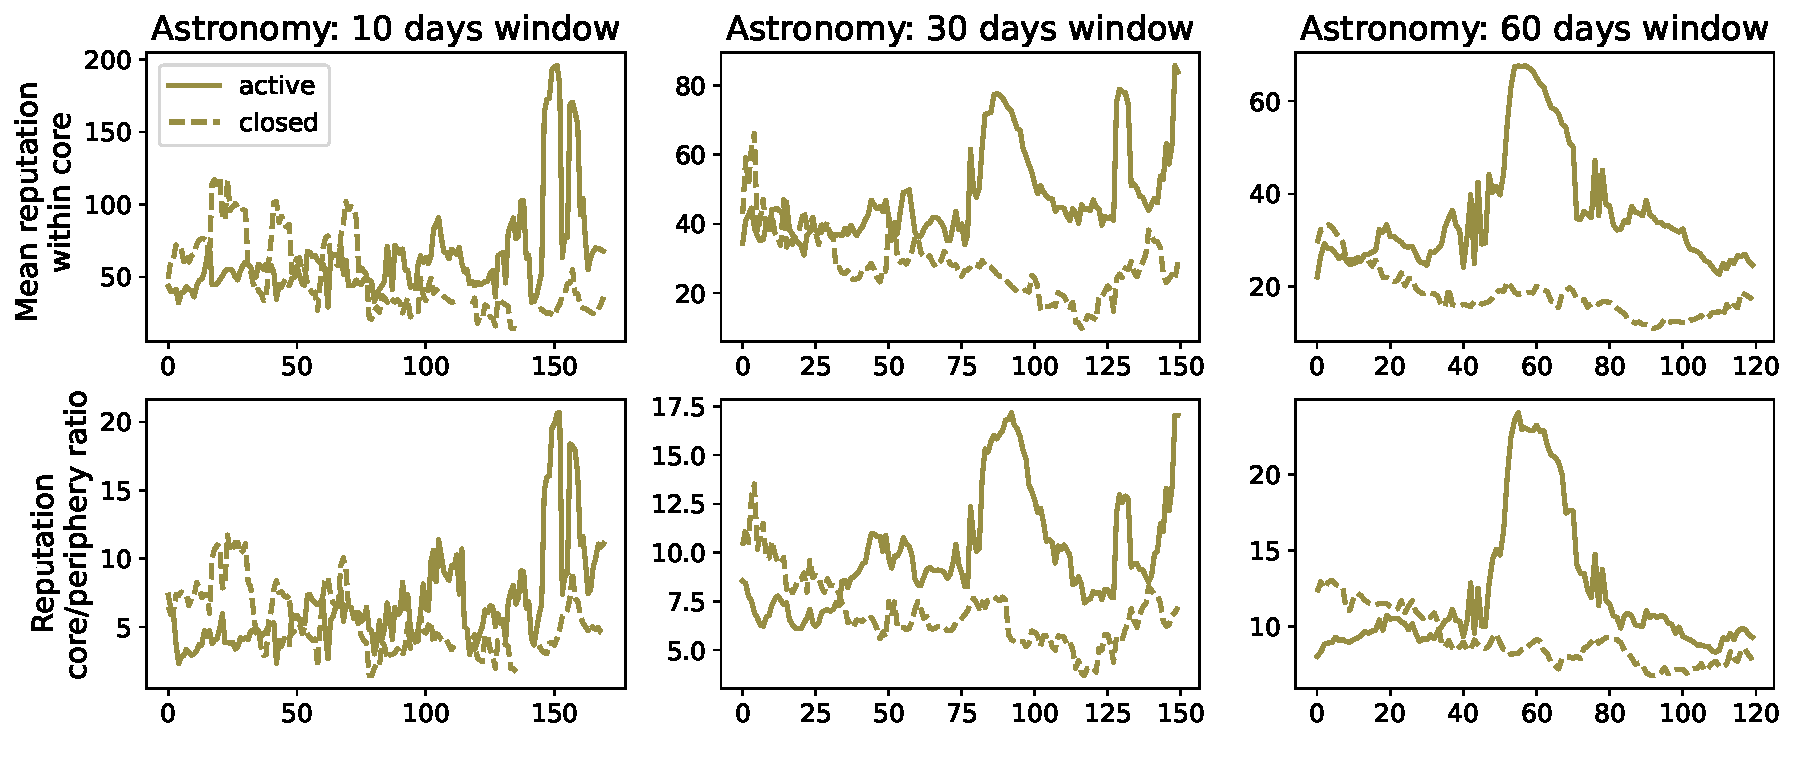
\includegraphics[width=\linewidth]{figures/stackexchange/sliding_window_core_reputation.pdf}
	\caption{Results for different sliding windows. Example is for astronomy, blue solid lines- active, orange dashed lines - closed site. }
	\label{fig:windows}
	% Ovo je mozda previse grafika, pa je mozda podeliti na dva dela. 
	% Ovo je primer za astronomiju (ali ako se odlucimo za neku drugu moze se zameniti)
\end{figure}
